\section{Les bas fonds de Taris}

\subsection{Résumé des épisodes précédents}
Nos héros se retrouvent donc dans un Cargo léger YZ-775 sans canons fonctionnel et un message entrant d’une inconnue qui demande à parler à Tinon.

Ils ont aussi apris qu’Industrial Automaton sous couvert d’expérimentations de son nouveau modèle, fait des recherches sur un très ancien artefact Sith en provenance de \textbf{Taris}. De plus, s’ils ont réussi à récupérer le droïde, Vyna Anen les attend sur l’avant-poste commercial de \textbf{l’anneau de Kafrene} au Starlord Café. Enfin, ils savent aussi que le vaisseau se dirigeait vers \textbf{Gaulus} pour rejoindre un laboratoire de l’empire où il devait finir des recherches sur l’artéfact.

Plusieurs directions s’offrent alors à nos héros.

\subsection{Les bons, les brutes ou les truants}
\begin{quotebox}
    Tinon \emph{(prononcer Taïnon)} c’est toi ? Que se passe t’il ou va tu ?
\end{quotebox}
Le visage d’une jeune femme apparait sur l’holocomm. Les héros ont le choix de répondre ou non.

Ce point de l’aventure est crutial pour nos héros car ils vont choisir (en connaissance de cause ou non) l’orientation de leurs personnages. En effet plusieurs cas de figures se présentent :

\begin{description}
    \item[\nameref{sec:les-rebels}] Répondre au message et suivre les consignes des Rebels (page~\pageref{sec:les-rebels}).
    \item[\nameref{sec:retour-du-droide}] Ramener le droïde à Vyna Anen (page~\pageref{sec:retour-du-droide}).
    \item[\nameref{sec:refus-d-obtemperer}] Partir pour Taris directement (page~\pageref{sec:refus-d-obtemperer}).
    \item[\nameref{sec:l-empire}] Prendre la direction de Gaulus (page~\pageref{sec:l-empire}).
\end{description}

Tous ses choix amèneront, de toute façon, les héros sur Taris mais le chemin sera différent et par là même leur orientation aussi. Je vais tacher de décrire les choix possibles sachant que rien n’est écrit dans le marbre et vous pouvez très bien les forcer suivre une route en particulier. C'est un peu le jeu de piste, les choix s'entrecroisent alors faut suivre. Mais une fois de plus rien n'est définitif, les joueurs auront toujours des idées farfelues auquelles on a pas pensé mais je vais essayé de décrire les principales voies possibles, au MJ de diriger les joueurs vers une de ces voies.


\subsubsection{Retour du droïde} \label{sec:retour-du-droide}

Autre choix possible pour les héros, ces derniers, avident de crédits, veulent allez rendre le droïde et récupérer le solde promis pour leur mission. Il retournent donc sur l'avant-poste commercial dans \textbf{l'anneau de Kafrène} ou les attend \nameref{sec:vyna-anen}.

On laisse les héros discuter un peu et réclamer leur due, Vyna acquiesce avec le sourire, leur donne les crédits mais au moment de quitter la pièce, 4 ou 5 \textit{(doser en fonction du niveau de vos joueurs)} Stormtroopers leur barre la route. Attention, à moins que les héros est anticipé, le premier tour de combat sera pour dégainer.

\begin{quotebox}
    Vous pensiez réellement qu'avec tout ce que vous savez, nous allons vous laisser repartir tranquillement ?\\
    Commencez par me rendre les crédits.
\end{quotebox}

Les héros peuvent tenter de négocier avec Vyna, ce dernier acceptera de les laissé repartir vivant (mais sans crédit) à condition qu'ils retourne sur \nameref{sec:taris} et recupèrent les informations que les scientifiques de Industrial Automaton n'ont pas eu le temps de récupérer. Ils peuvent tenter un jet de Négociation pour garder les crédits.\\

Si les héros entrent en combat, et qu'ils perdent, on ne les tue pas mais Vyna leur impose de retourner sur Taris et pas de négociation possible. S'ils gagnent, deux cas de figure possible :
\begin{rebelist}
    \item \textbf{Ils tuent Vyna} Un homme, dathomirien, manifestement important en uniforme de l'empire entre dans la pièce en applaudissant. Pausément, il félicite les joueurs et   leur expliquent qu'il ont réussi le test avec brillo. Vyna était devenu génant pour l'empire et pour l'Odre. Si l'un des héros tente quoi que ce soit il se retrouve désarmé et collé au mur avant d'avoir eu le temps de comprendre. On déccroche sur \nameref{sec:l-empire}.

    \item \textbf{Ils laisse Vyna en vie} Une femme (celle qui est apparue sur le holocom du vaisseau) entre dans la pièce avec deux hommes. Les deux hommes emportent Vyna avec eux, en faisant comme s'il était ivre. Et la femme leur fait signe de la suivre vite, elle leur expliquera plus tard. Ils prennent le vaisseau et partent pour la cache des Rebels. On déccroche sur \nameref{sec:les-rebels} dans la version bien accueilli.
\end{rebelist}

Le \nameref{sec:nimbus} n'est réparé qu'à leur demande, le prix est de 40 000 \crg. Négociable à 30 000, -10k si relance.


\subsubsection{Les rebels} \label{sec:les-rebels}

\begin{quotebox}
    Tinon \emph{(prononcer Taïnon)} c’est toi ? Que se passe t’il ou va tu ?
\end{quotebox}

Le visage d’une jeune femme apparait sur l’holocomm et les héros choisissent de répondre.

\begin{quotebox}
    Mais qui êtes vous et où et Tinon ?
\end{quotebox}
Les joueurs choisissent de raconter leur histoire, ou de mentir, à voir ce qu'ils préfèrent. Lindi leur demande de la rejoindre et leur donne les coordonnées d'une cache de la Rébellion. Si les joueurs ont menti, il sont accueilli avec suspicion, menacé et tout ce qui va avec, sinon ils sont accueillit normalement avec juste un peu de méfiance. \textbf{Lindi Dangon} les invite à la suivre et les interroge jusqu'à ce qu'ils disent la vérité (On part du principe que s'ils persistent à mentir, on bifurque vers l'option \nameref{sec:refus-d-obtemperer}).

Lindi leur explique alors que la résistance à eu vent des recherches mené par l'Industrial Automaton ainsi que des problèmes sur le Pelican. \textbf{Tinon Dystra} avait été envoyé pour tenté de s'infiltrer à bord du Pelican. Mais qu'il n'avait plus donné de nouvelles depuis son arrimage au vaisseau.

Un jet de \textbf{Perception} ou l'utilisation de \textbf{Sens de Force} fera apparaître les sentiments de Lindi envers Tinon et apprendra à nos héros que ces derniers étaient amants.\\

Une fois la discution terminé, Lindi demande de l'aide aux héros, qu'ils reprenne le travail de Tinon. La première piste à explorer étant \ldots \nameref{sec:taris}.

Le \nameref{sec:nimbus} est réparé gratuitement pendant que les héros discutent.


\subsubsection{Refus d’obtempérer} \label{sec:refus-d-obtemperer}

Les héros veulent se la jouer et décident de partir direct sur Taris. Mais ils ne savent même pas trop se qu'ils y cherche. L'hyper-espace est récalcitrant et ne veut pas fonctionner immédiatement. Le temps de regarder, un croiseur sort d'hyper-espace et les arraisonne sans poser de question. Des soldats de l'alliance (trop pour être combattu) forcent la cloison et entre dans le cargo, suivi par la femme vu précédemment sur l'holocomm.

\begin{quotebox}
    Où pensiez vous partir comme ça avec ce cargo ? \\
    \emph{se retournant vers les soldats}, jetez moi ça en cellule on les interrogera là bas.
\end{quotebox}

Les héros sont transporté jusqu'à une cache de la Rébellion et jeté en cellule. Au bout de quelques temps, la femme précédement rencontré vient les interroger. Ils ont le choix de répondre la vérité ou de mentir. S'ils répondent la vérité, on déccroche sur l'option correspondante dans \nameref{sec:les-rebels}. Sinon ils sont laissé en cellule \ldots

Mais dans la nuit, un mystérieux inconnu s'approche de la cellule sans bruit

\begin{quotebox}
    Je suis envoyé par Vyna Anen, si vous voulez vivre, venez avec moi et ne faites pas un bruit.
\end{quotebox}

L'inconnu ouvre leur cellule et les emmène au Cargo. Sur le chemin, leur demander des jets de \textbf{Discrétion}. En cas d'échec deux soldats débarquent. Dans le hangar où se trouve le Cargo, 4 soldats montent la garde. Soient les héros passent en force et débute un combat puis vont ouvrir les portes du hangar. Soit ils la jou furtif, se glissent dans le vaisseau et tire sur les portes pour sortir du hangar. Ou n'importe quoi d'autre qui leur permet de sortir. Une fois dehors l'inconnu leur transmet des coordonnées. Ils n'ont pas le choix, s'ils font mine de résister, l'inconnu sort une arme et les tiens en joue. Eux n'ont pas d'arme ils sortent de cellule. On déccroche ensuite sur \nameref{sec:l-empire}.



\subsubsection{L’empire} \label{sec:l-empire}
Enfin, dernière alternative les héros peuvent vouloir partir pour \textbf{Gaulus} la planète vers laquelle se dirigeait le vaisseau. 

A l'approche de la planète, le cargo est arraisonné par un croiseur de l'empire. Les héros sont invité à sortir et une dizaine de Stormtroper les attendent. Ils sont escroté jusque dans un bureau où les attendant \nameref{sec:vyna-anen} et un Dathomirien en uniforme de gradé de l'empire. C'est ce dernier qui prend la parole.

\begin{quotebox}
    Messieurs (mes dames) nous vous attendions. Asseyez vous je vous pris. \\
    Alors comment s'est passé cette mission, je vois que tout le monde n'est pas revenu \emph{(sourire aux lèvres)}. 
\end{quotebox}

Le droïde est emmené par deux gardes. Puis le Dathomirien se présente.

\begin{quotebox}
    Je me présente, je m'appelle \nameref{sec:garan-keggle}, j'ai suivi la mission de loin et je tiens à vous féliciter, vous vous en êtes sorti plutôt bien. Je pensais pas que vous viendriez à bout de l'Amblyope mais j'avoue que le combat était intéressant. Au vue de vos qualités respective, je souhaiterais que vous partiez pour \nameref{sec:taris} afin de finir la travail \emph{(il jette un regard froid sur Vyna qui en même pas large et baisse les yeux)} nous avons besoin de plus d'information sur la position de l'artéfact.
\end{quotebox}

Si les héros se hasard à demander un prime, on leur répond que l'empire saura les récompenser sans plus de détail. S'il sont récalcitrant on leur explique que c'est pas une proposition que l'on vient de leur faire.


\subsection{Taris} \label{sec:taris}
\noindent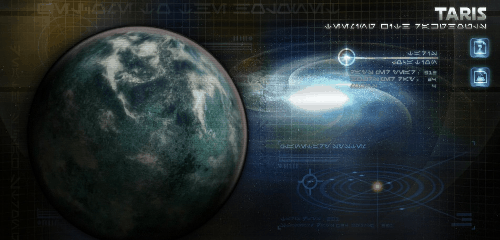
\includegraphics[width=\linewidth]{_img/dos-au-muur/taris.png}
Taris est une planète urbaine, très polluée, de la Bordure Extérieure. Divisée en trois grandes parties en fonction des étages, la Ville Haute, la ville basse et les "bas fonds", elle abritait autrefois une population gigantesque. Grand pôle économique dans la galaxie, notamment grâce à l’implantation des industries Lhosan, elle joignit la République Galactique peu avant les Guerres Mandaloriennes. Mais après la passage de Dark Malak plus de 4000 ans auparavant la planète à du mal à reprendre vie. Les "bas fonds", qui abritaient toutes sorte de hors la loi et de rebus de la société, est la partie de Taris qui s'en est le mieux sortie et c'est pourquoi les ruines marécageuses de Taris sont très dangeureuses. La république a depuis implanté un spaciaux port et une base militaire sur la planète dans l'espoir de la recoloniser mais le processus s'avère lent et compliqué.

Normalement une fois au spacioport, vos héros ne savent pas où aller. Plusieurs choix s'offre à vous pour les orienter. Est de leur placer un bar bien en évidence sur leur chemin. A l'intérieur ils pourront trouver des informations et peut être même un guide.

Normalement, ils vont se diriger vers le barman. Au pire, c'est le barman qui vient à eux pour leur demander ce qu'ils veulent boire. Ce dernier, un Besalisk, leur explique que l'endroit où ils souhaite se rendre (les ruines de l'ancien temple Sith) se trouve dans un zone interdite, au coeur de la zone de quarantaine \nameref{sec:rakghoul}. Il n'est pas possible de s'y rendre.

Mais un client du bar les accoste et leur dit que moyennant 20 000 \crg il les conduira où ils le souhaite. Un jet de négociation (opposé à la négociation de l'inconnu 5) fera descendre la somme à 15 000 \crg.

\subsubsection{Quête annexe (optionnel)}
Il est possible d'intégrer une petite quête annexe ici histoire de varier les plaisirs. S'ils la réussisse on pourra distribuer +1 XP supplémentaire.

L'inconnu propose à vos héros de les conduire gratuitement aux ruines s'ils l'aide. Selon l'orientation des joueurs à ce moment, soit:
\begin{description}
    \item [obscur] Ils aident un contrebandier à Kidnapper une jeune Twi'lek répéré dans un camp de réfigié pas loin.
    \item [clair] Ils aident un père à délivrer sa fille Twi'lek des mains de contrebandiers.
\end{description}

Le roleplay est un peu différent selon la situation mais la quête se déroule de la même façon. Les héros suivent l'inconnu qui s'est présenté entre temps (\nameref{sec:gil-harend}). Ce dernier les conduit au camp (de réfugiés ou de contrebandier). Un jet de Discretion réussi par tout le monde permet de s'approcher de la cible. Un jet de discrétion réussi par tous permet de s'extraire de camp sans encombre. Le joueur qui est chargé de transporté la cible à un malus de -2 à son deuxième jet de discrétion.

Si une Discrétion est raté par l'un des joueurs, un combat commence. Vos héros se trouve confronté à H -1 contrebandiers/réfugiés (H est le nombre de joueurs que vous avez). Vos héros ont l'initiative sur le premier round. En face les ennemis ont les caractéristiques \nameref{sec:taris-contrebandier}.

Attention, \nameref{sec:gil-harend} ne doit pas mourir sinon la quête est un échec et retour au bar. 

\subsubsection{Les ruines de l'ancien temple Sith}
\noindent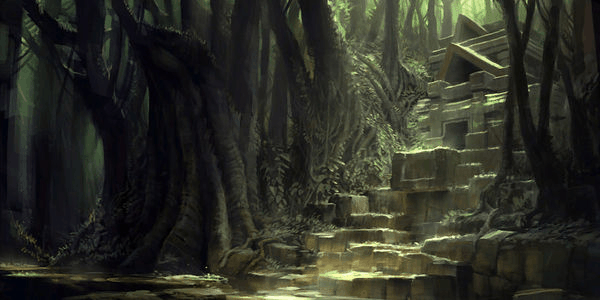
\includegraphics[width=\linewidth]{_img/dos-au-muur/taris-temple-sith.png}

Après plusieurs heures de marche dans les marécages de Taris, le groupe arriver devant les ruines de l'ancien Temple Sith. Le côté obscur de la Force émane du temple dans toutes les directions et l'atmosphère est pesante. D'ailleurs on entend absolument aucun bruit, comme si toute la faune avait déserté la zone. L'entrée est partiellement éboulée mais il reste une ouverture suffisante pour s'y faufiler.

Après être entré dans le temple les héros se retrouvent dans une immense salle, très haute de plafond. Deux rangées de statues de 10m de haut représentent d'anciens seigneurs Sith (Un jet de Connaissance (Sith) permet d'apprendre qu'il s'agit de Tulak Hord, Dakhan Shar, Naga Sadow, \ldots entre autres). Au fond de la salle une fresque murale est gravée sur un monolithe.

Chacun des murs de la pièce (en dehors de celui de l'entrée dans leur dos) possède deux ouvertures vers des pièces.

Devant le monolithe, les vestiges d'un campement de fortune (attention, c'est des vestiges de 3000 ans quand même, heureusement à l'époque on faisait les choses pour que ça dure ;-) ) recouvert de poussière. Une partie de ce campement semble pourtant avoir été remué récemment.

Naturellement, nos héros ne sont pas seul. 5 \nameref{sec:rakghoul} débarquent et encerclent les héros, s'en suit une phase de combat.
\\

Une fois les Rakghoul élliminés, les héros peuvent aller observer le monolithe et le campement.

<<insérer le dessin de la fresque>>

Un jet de \emph{Connaissance (Sith)} permet de comprendre la fresque. 

\begin{quotebox}
6 000 ans par le passé, un Jedi fut exilé pour ses penchants obscur et ses expériances interdites sur la vie. Son objectif était, en utilisant le coté obscur, de pouvoir plier la vie elle même à sa volonté et ainsi acquérir la vie éternelle. En étudiant l'alchimie du coté obscur il parvient à créer un Talisman renfermant son essence et sa volonté. Cet artéfact devait, entre autre, lui permettre de prendre posséssion du corp du porteur du Talisman mais aussi de contrôller les Rakghoul.

Ce Jedi Noir fut tué par un de ses rivaux et durant les décennies suivantes plusieurs Seigneurs Sith se déchirèrent entre eux afin de mettre la main sur ce Talisman. Enfin, l'artéfact et son porteur du moment finirent par être tué et enseveli dans ce temple au milieu des bas-fonds de Taris.
\end{quotebox}

S'ils ne font pas ce jet ou qu'ils le ratent, il ne peuvent que tenter d'interpréter la fresque. Après il leur est possible de faire des recherches sur cette fresque dans un temple Jedi ou une bibliothèque. En soit l'histoire n'a pas une grosse importance pour la suite, c'est un bonus pour eux.

Si l'un des héros possède vision de force et s'en sert, il pourra distinguer sur le monolithe un texte, le code des Sith écrit en lettres obscures
\begin{quotebox}
La paix est un mensonge, il n’y a que la passion. \\
Par la passion, j’ai la puissance. \\
Par la puissance, j’ai le pouvoir. \\
Par le pouvoir, j’ai la victoire. \\
Par la victoire, je brise mes chaînes. \\
La Force me libérera.
\end{quotebox}
\\

Ensuite avec un jet de recherche sur le campement de fortune, ils trouvent un vieux datapad mais qui a besoin d'être chargé. Dommage, personne n'a de quoi l'alimenter sur lui (sauf si quelqu'un possède l'Atout \emph{Recycleur} et s'en sert). Il faudra trouver le matériel et faire un jet de \emph{Réparer} pour en tirer des informations.

Dans les autres pièces du temple si les héros éffectuent une recherche ils ne trouvent rien que des restes de Rakghoul et d'animaux à moitié dévorés.
A la sortie du temple, les héros sont attendu de pied ferme par 3 \nameref{sec:taris-contrebandier}s. C'est soit les contrebandiers à qui il s ont repris la jeune fille plus tôt qui viennent se rembourser. Soit les amis de \nameref{sec:gil-harend} qui a décidé de les doubler. Dans tout les cas, les contrebandiers veulent récupérer le datapad. Baston\ldots

Une fois débarrassé des contrebandiers, retour au spacioport où ils trouveront de quoi réparer le datapad et en tirer les informations qu'ils cherchent.

Le datapad appartenait à un certain \nameref{sec:pulsipher} qui en étudiant les archives du temple Jedi de Taris avait apris l'existence de l'artéfact. D'après les informations, Pulcipher a procédé à des excavations et a trouvé le Talisman de Muur. Mais il du plier bagage rapidement car 3 Jedis appartenant au Cercle de Veille de Taris arrivent pour récupérer le Talisman. Pulcipher quitte alors Taris à bord du Mar'eyce, qui prit la direction de \textbf{Jebble}

\subsection{Nimbus} \label{sec:nimbus}
Cargo léger YZ-775

-----


Bon l'idée c'est que dans tout les cas la prochaine étape est Taris et le temple Sith dans lequel ils trouverons un holocron qui leur dira que le Talisman est partie sur Jebble avec Céleste Morne et Pulcipher.
L'holocron parle de l'oubliette de Dreypa et de la rivalité entre Dreypa et Karness. Il ne dit pas ou se trouve l'oubliette ni le talisman. 
Pas loin se trouve les restes du campement de Pulcipher avec son journal qui explique qu'il a l'intention de partir pour Jebble à son labo pour y étudier l'artéfact. Le dernier message est coupé avant la fin mais il semble que Pulcipher et été interrompu par un duo de Jedi et ai du quitté Taris en précipitation.


L'épisode suivant se passe sur Jebble dans le labo du professeur Pulcipher. Où l'on apprend ce qu'il s'est passé pendant le voyage de retour et où l'on a des piste sur l'endroit ou se trouve l'oubliette. On entend notement parler de Céleste Morne.
Ici une idée est qu'au moment de quitté la planète pour l'étape suivante, les héros se retrouvent pris au piège par des troupes de l'empire qui on pris leur vaisseau en otage. Histoire de varier l'aventure. On peut même se mettre une petite baston spaciale.
Il faudra ensuite forcer les héros à retourner à leur QG (alliance rebelle ou empire) pour réparation et pour compte rendu.

Dans l'épisode suivant, le rebelles apprennent qu'on aurait vu le talisman sur une certaine lune de Jesaispasou et les soldats de l'empire apprenne qu'ils vont tendre un piège à l'alliance sur un lune de Jesaispasou.
Grossomerdo, Celeste se pointe et calme tout le monde, obligé de battre en retraite et de trouver un plan pour enfermer Celeste dans l'oubliette de Dreypa ou pour lui virer le Talisman avant d'enfermer ce dernier dans l'oubliette. Ou se trouve l'oubliette ? Quel est le plan ?